\chapter{System Design}
\label{ch:design}
% ============================================================

\section{System Architecture}
\label{sec:architecture}

The system is organised into five layers with explicit interface contracts between
them. Layer separation is deliberate: the simulation layer is replaceable by captured
traces from a hardware testbed, and the detection layer is replaceable by a different
model, without either change propagating beyond its own interface.

\begin{figure}[htbp]
\centering
\begin{tikzpicture}[
  layer/.style={draw, rounded corners=2pt, minimum width=11cm, minimum height=1.05cm,
                align=center, font=\small},
  iface/.style={font=\scriptsize, align=center},
  node distance=1.05cm
]
\node[layer] (l1) {\textbf{L1 Simulation Layer} \\
  \scriptsize Zonal TSN topology, gPTP synchronisation, attack injection, seeded execution};
\node[layer, below=of l1] (l2) {\textbf{L2 Observation Layer} \\
  \scriptsize Passive capture of per-node timing state; no forwarding-path involvement};
\node[layer, below=of l2] (l3) {\textbf{L3 Feature Layer} \\
  \scriptsize Windowing, residual computation, labelling, dataset export};
\node[layer, below=of l3] (l4) {\textbf{L4 Detection \& Federation Layer} \\
  \scriptsize Local training, FedAvg aggregation, inference, confidence};
\node[layer, below=of l4] (l5) {\textbf{L5 Alerting \& Presentation Layer} \\
  \scriptsize Attributed alerts, incident queue, metric export};

\draw[-{Latex[length=2mm]}] (l1) -- node[right, iface] {\;IF-1: raw per-node vectors} (l2);
\draw[-{Latex[length=2mm]}] (l2) -- node[right, iface] {\;IF-2: time-ordered signal series} (l3);
\draw[-{Latex[length=2mm]}] (l3) -- node[right, iface] {\;IF-3: \texttt{features.csv} schema} (l4);
\draw[-{Latex[length=2mm]}] (l4) -- node[right, iface] {\;IF-4: alert record} (l5);
\end{tikzpicture}
\caption{Layered system architecture with interface contracts.}
\label{fig:arch}
\end{figure}

\section{Architectural Components}
\label{sec:components}

\begin{longtable}{p{0.18\textwidth} p{0.24\textwidth} p{0.5\textwidth}}
\toprule
\textbf{Component} & \textbf{Layer} & \textbf{Responsibility} \\
\midrule
\endhead
Topology model & L1 & Declares nodes, links and per-node clock configuration \\
Scenario manager & L1 & Schedules attack events at configured times and targets \\
gPTP instances & L1 & Distribute time from the grandmaster through the relay tree \\
Signal recorder & L2 & Records per-node clock state at sample points \\
Window builder & L3 & Segments series into fixed-size observation windows \\
Feature computer & L3 & Computes per-window statistics and residuals \\
Labeller & L3 & Assigns class and zone attribution from the ground-truth record \\
Local trainer & L4 & Trains the shared model architecture on a client's local dataset \\
Aggregator & L4 & Performs FedAvg over received parameters \\
Inference engine & L4 & Classifies windows using the deployed global model \\
Fallback detector & L4 & Rule-based detection when no valid model is available \\
Alert builder & L5 & Constructs attributed alert records \\
Incident queue & L5 & Operator-facing triage surface \\
\bottomrule
\end{longtable}

\section{Interfaces and Dependencies}
\label{sec:interfaces}

\begin{longtable}{p{0.08\textwidth} p{0.26\textwidth} p{0.58\textwidth}}
\toprule
\textbf{ID} & \textbf{Interface} & \textbf{Contract} \\
\midrule
\endhead
IF-1 & Simulation $\rightarrow$ Observation &
Per-node recorded vectors in the simulator's result format; one vector per node per
run; node identity encoded in the vector name \\
\addlinespace
IF-2 & Observation $\rightarrow$ Feature &
Time-ordered $(t, \text{value})$ series per node, with run identifier and seed \\
\addlinespace
IF-3 & Feature $\rightarrow$ Detection &
\texttt{features.csv} column contract (Table~\ref{tab:schema}); one row per window per
zone; stable column order; documented units \\
\addlinespace
IF-4 & Detection $\rightarrow$ Alerting &
Alert record: \{class, confidence, zone, window start, window end, run id,
supporting feature values\} \\
\addlinespace
IF-5 & Client $\leftrightarrow$ Coordinator &
Model parameters and training metadata (sample count, round index). Feature records
are explicitly excluded from this interface (NFR-07) \\
\bottomrule
\end{longtable}

\textbf{External dependencies.} OMNeT++ 6.4.0 (simulation kernel, Qtenv/Cmdenv),
INET 4.7.0~\cite{inettsn} (TSN and gPTP modules), Python 3 with scientific stack for extraction and
training, and a federated learning framework for the aggregation layer. Versions are
pinned in Section~\ref{sec:dependencies}.

\section{Architecture Decisions and Rationale}
\label{sec:arch-decisions}

\begin{longtable}{p{0.06\textwidth} p{0.26\textwidth} p{0.26\textwidth} p{0.34\textwidth}}
\caption{Architecture decision record}\\
\toprule
\textbf{ID} & \textbf{Decision} & \textbf{Alternatives considered} & \textbf{Rationale} \\
\midrule
\endfirsthead
\toprule
\textbf{ID} & \textbf{Decision} & \textbf{Alternatives considered} & \textbf{Rationale} \\
\midrule
\endhead
AD-1 & Use OMNeT++/INET as the simulation framework &
Build a custom simulator; use a hardware TSN testbed; use a generic network simulator
without TSN modules &
INET provides gPTP, time-aware shaping and clock-drift modelling as maintained
components, and its TSN capabilities have been verified against TSN hardware
measurements in published work. Building a simulator would consume the project budget
without advancing the research question. A hardware testbed is unavailable and its
procurement risk is unacceptable within the timeline. \\
\addlinespace
AD-2 & Supervised multiclass classification &
Unsupervised (LOF, autoencoder, Deep SVDD); two-stage hybrid &
Simulation supplies ground-truth labels, removing the label-scarcity constraint that
motivates unsupervised framing in the comparable literature. A parametric model has
trainable weights and is therefore FedAvg-compatible without a non-standard
aggregation scheme; LOF is not. LOF is retained as a comparison baseline for
comparability with published results. \\
\addlinespace
AD-3 & Federate across zones within one vehicle &
Federate across vehicles/fleet &
The aggregation server is the vehicle's own central compute unit. Within-vehicle
federation is motivated by backbone bandwidth, not inter-organisational privacy:
periodic fixed-size parameter exchange is a bounded, schedulable traffic pattern,
whereas continuous trace upload is unbounded best-effort traffic competing with
protected streams. \\
\addlinespace
AD-4 & Static, one-shot training &
Continuous/online federated learning &
Online retraining in deployment requires live ground-truth labelling, which has no
solution within scope. Assumption A2. \\
\addlinespace
AD-5 & Static network environment assumption &
Support runtime reconfiguration &
The detection approach computes residuals against an expected value known from
configuration. This is available \emph{a priori} only when the configuration is
static. Supporting dynamic reconfiguration requires distinguishing legitimate
reconfiguration from attack, which is a separate research problem. Assumption A1. \\
\addlinespace
AD-6 & Detector positioned at the zone controller &
Position at endpoint ECU; position centrally &
The primary features require simultaneous visibility of multiple ports: the sibling
offset residual cannot be computed by a node that observes only its own clock. The
zone controller is the lowest point in the hierarchy with the required visibility. \\
\addlinespace
AD-7 & Flat CSV dataset with a documented column contract rather than a relational
schema &
Relational database with entity-relationship model &
The data is a single homogeneous observation table with no multi-entity relational
structure. A relational model would add no referential integrity benefit and would
not reflect the domain. Section~\ref{sec:data-design} therefore specifies a column contract rather than
an ERD. \\
\bottomrule
\end{longtable}

\section{Reference Topology Design}
\label{sec:ref-topology}

The Iteration~1 results reported in Chapter~\ref{ch:testing} were produced on a four-zone tree
topology, described in Section~\ref{sec:technical-details} and retained as \texttt{topology\_basic}. That
topology was built to be minimal: it was enough to instrument gPTP, inject delay
attacks and test the cross-zone residual claim, and deliberately no more. It has two
properties that bound what can be asked of it. Each zone reaches the backbone over a
single path, so FRER cannot be configured, and all four zones carry identical traffic,
which is recorded as defect DEF-02.

A second topology, \texttt{topology5}, has since been designed and generated to remove
both limits. It is the reference topology for the remainder of the project. It has
been validated structurally but has not yet produced a dataset, so no result in this
report is derived from it.

\subsection{Basis of the design}
No vehicle manufacturer publishes harness or ECU-placement data, so the topology is
built as a representative reference rather than a copy of a production vehicle. Three
published sources inform it. The zone-based in-vehicle architecture evaluated in
\emph{Sensors}~\cite{park2023zonal} supplies the organising principle: ECUs are grouped into zones
by physical location, attached to the nearest zone controller, with a central compute
unit as the inter-zone hub. The TSN anomaly-detection assessment framework of
Meyer, H\"ackel, L\"ubeck, Korf and Schmidt~\cite{meyer2024framework} supplies a precedent for a
ring-based zonal topology carrying
corner lidar, front and rear cameras, infotainment, a connectivity gateway, a gPTP
master and an ADAS unit, modelled in OMNeT++/INET. Industry material on zonal E/E
architecture, including the IEEE~802 zonal presentation and Excelfore's TSN wheel-sensor
work, supplies the four-corner-plus-cabin arrangement and the use of TSN for
time-critical traffic with network redundancy. The device list is the project's own
representative model and is not claimed to match any production vehicle.

\subsection{Zone partitioning}
The vehicle is divided into five zones: front-left (FL), front-right (FR), rear-left
(RL), rear-right (RR) and a centre/cabin zone (C). Each zone has one TSN switch and
one zonal controller host, and the controller is the node that runs the local detector
and acts as the federated client. Devices are assigned to zones by three rules applied
in order: physical proximity, so a device connects to the switch of the zone in which
it is mounted; safety separation, so safety-critical actuators such as steering and
brake are kept apart from infotainment and external-facing nodes; and a load limit, so
a zone's uplink load stays within the capacity of its links, with devices moved or link
speed revisited if it does not.

The model contains 25 endpoint ECUs, five zonal controllers, a central compute unit, a
connectivity gateway and a gPTP master clock.

\begin{longtable}{p{0.16\textwidth} r p{0.56\textwidth}}
\caption{Zone composition of the reference topology}\label{tab:topology5}\\
\toprule
\textbf{Zone} & \textbf{ECUs} & \textbf{Examples} \\
\midrule
\endfirsthead
\toprule
\textbf{Zone} & \textbf{ECUs} & \textbf{Examples} \\
\midrule
\endhead
Front-left & 7 & lidar, radar, front camera, left mirror camera, steering, brake,
front ultrasonic \\
Front-right & 6 & lidar, radar, right mirror camera, powertrain, ultrasonic,
headlamp \\
Rear-left & 3 & lidar, radar, ultrasonic \\
Rear-right & 4 & lidar, radar, rear camera, V2X unit \\
Centre/cabin & 5 & infotainment, instrument cluster, driver-monitoring camera,
audio amplifier, GNSS receiver \\
\bottomrule
\end{longtable}

The distribution is deliberately uneven. The front zones carry dense sensing and
control traffic, the rear zones are lighter, and the cabin zone carries mainly
multimedia and display traffic. The ECU count was chosen for this project rather than
copied from the source architecture: enough devices per zone to give each federated
client a meaningful local dataset, while keeping the simulation maintainable.

\subsection{Interconnect}
Within a zone, devices connect to the zone switch in a star. Between zones, the four
corner switches form a ring (FL, FR, RR, RL) and the centre switch is dual-homed to
both front switches. Every zone therefore has two link-disjoint routes to the centre,
which is precisely the property that Frame Replication and Elimination for Reliability
requires and which the earlier tree topology could not provide. Ring links and ADAS
sensors run at 1~Gbps; lower-rate ECUs run at 100~Mbps. Link lengths of 0.5 to 3.5~m
are assumed values chosen to be plausible for a passenger vehicle and are kept below
the 15~m reach of automotive Ethernet over unshielded twisted pair.

The ring is the primary topology because it enables FRER-based detection features and
path-change behaviour in gPTP. A star topology over the same device inventory is
retained as a baseline for comparison, since a star offers only one path per zone and
therefore isolates what the redundancy actually contributes.

\subsection{Time synchronisation}
A gPTP grandmaster is attached to the centre switch. Synchronisation follows a static
tree: grandmaster, centre switch, front switches, rear switches, then end devices. The
two ring links not on this tree (FL to FR, and RL to RR) carry no synchronisation
messages. The simulator's gPTP implementation assigns master and slave ports statically
and has no best-master-clock algorithm, so a backup grandmaster is not modelled within
the current scope. gPTP and FRER are the two TSN signals used for detection.

\subsection{Generation and reproducibility}
The network description (\texttt{.ned}), the simulation configuration
(\texttt{omnetpp.ini}) and the validation checks are all generated from a single Python
table of devices, link speeds and link lengths (\texttt{gen\_topology.py}). Editing the
table and re-running the generator regenerates both simulator files, so the model
cannot drift out of step with its own specification, and the generation step runs in
the project's continuous integration pipeline (Section~\ref{sec:repository}).

\begin{figure}[htbp]
\centering
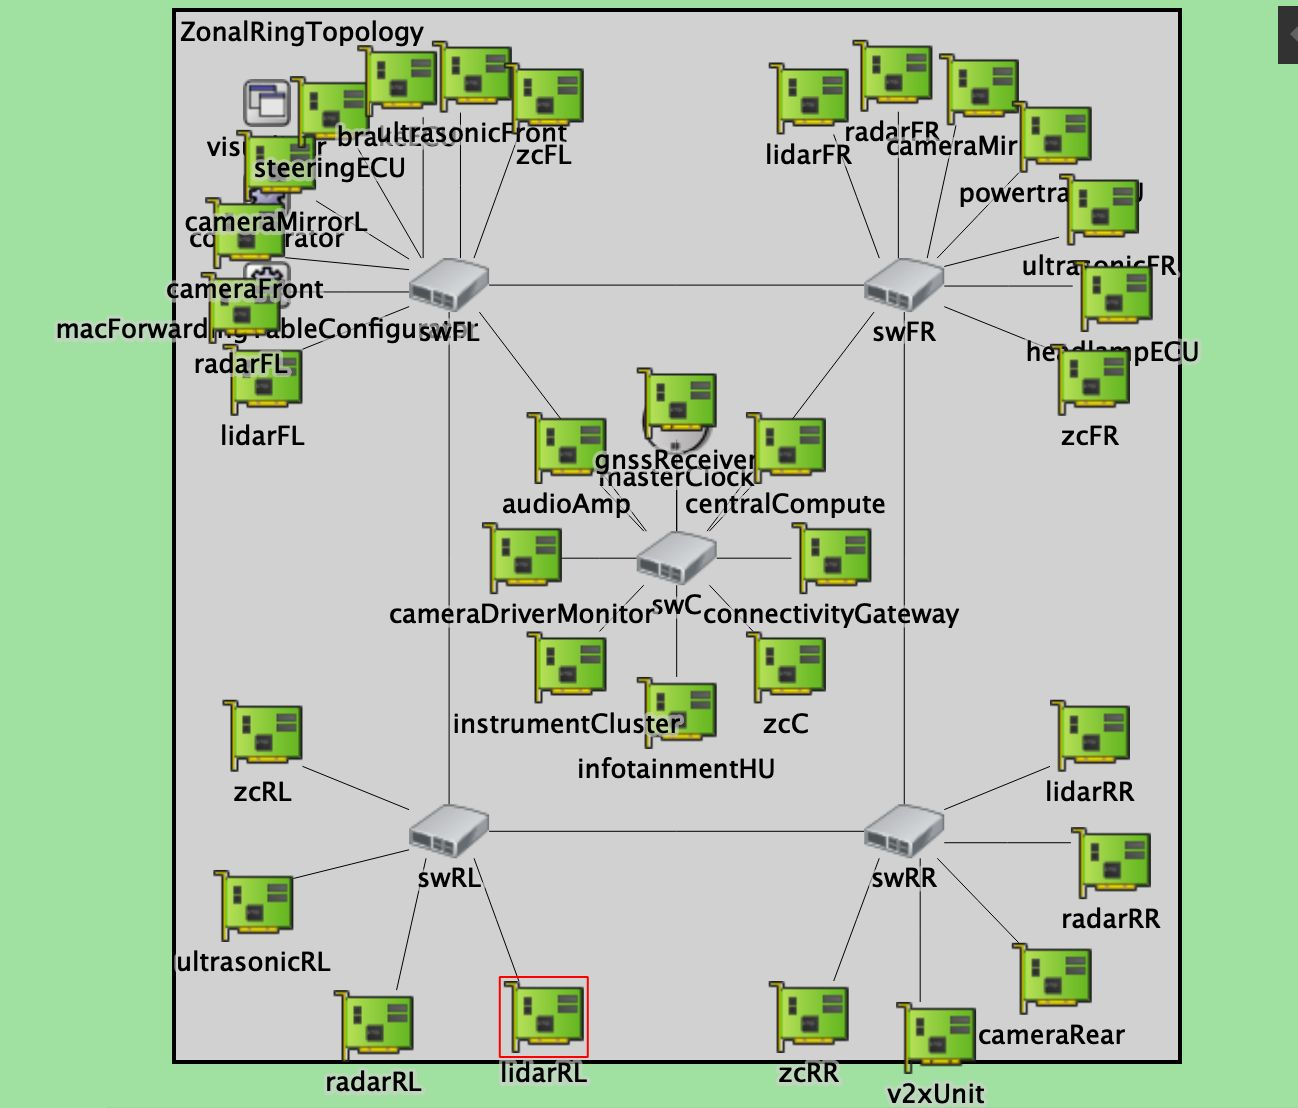
\includegraphics[width=0.95\textwidth]{figures/network_topology.jpeg}
\caption[Five-zone ring reference topology]{The five-zone ring reference topology (\texttt{ZonalRingTopology}) as
rendered in the simulator. The four corner switches \texttt{swFL}, \texttt{swFR},
\texttt{swRR} and \texttt{swRL} form the ring; the centre switch \texttt{swC} is
dual-homed to both front switches. Every zone therefore has two link-disjoint routes
to the centre, which is the property FRER requires. Each zone switch carries its own
zonal controller (\texttt{zcFL}, \texttt{zcFR}, \texttt{zcRL}, \texttt{zcRR},
\texttt{zcC}), which is the node that acts as a federated client, together with the
endpoint ECUs of that zone. The grandmaster (\texttt{masterClock}) and the central
compute unit are attached to \texttt{swC}.}\label{fig:topology5}
\end{figure}

\subsection{Validation}
\label{sec:topology-validation}
The topology is checked at three levels.

\textbf{Structural, automated.} The generator verifies that the graph is connected,
that each endpoint has exactly one switch port, that cutting any single ring or uplink
link partitions nothing, and that every link is shorter than 15~m. The current model
passes all of these checks. The partition check is the one that matters for FRER: it is
the machine-checkable form of the disjoint-path requirement.

\textbf{Physical plausibility, manual.} Each device is checked against the placement
rules: sensors connect to the switch of the zone in which they are mounted, cabin
devices connect to the front or centre zone, and safety-critical ECUs are kept separate
from infotainment. Each placement is justified by a source or a stated reason.

\textbf{Network behaviour, simulation.} The third level is specified here as the
acceptance criteria for the benign baseline run, which is the first task of
Iteration~03c (Section~\ref{sec:remaining-iterations}). The topology is accepted as behaviourally sound when all
time-triggered flows meet their deadlines, link utilisation stays below approximately
70\%, gPTP converges within the target bound, and FRER flows survive a cut ring link.
Stating these criteria before the run is deliberate: it fixes what counts as a
successful topology in advance, so that the baseline run tests the design rather than
being read as a description of whatever it happens to produce.

\subsection{Expected heterogeneity}
Each zonal controller acts as a federated client whose data is the traffic passing
through its zone switch. The topology is designed so that three kinds of non-IID
behaviour can arise across those clients: quantity skew, since zones differ in the
number of flows and therefore in the number of samples; feature skew, since traffic
classes, packet sizes and rates differ by zone and gPTP delay grows with hop distance
from the grandmaster; and label skew, since attack exposure differs by zone, with
V2X-related attacks reaching the rear-right zone and gPTP attacks affecting deeper
zones more strongly.

This is the designed remedy for defect DEF-02, which records that the four zones of the
earlier topology carry identical traffic and would make the federated comparison null
by construction. The remedy is a design property until it is measured. It will be
quantified by comparing per-zone feature distributions, using the
Kolmogorov--Smirnov statistic or the Wasserstein distance, and per-zone label
distributions, using the Jensen--Shannon divergence. Until those numbers exist, DEF-02
is reduced from open to partially addressed rather than closed.

\subsection{Limitations}
Four limitations are recorded against this topology. The device list and link lengths
are representative rather than taken from a manufacturer's vehicle. The model carries no
application traffic yet, so the heterogeneity described above is a design property and
not a measured one. gPTP is statically configured with no backup grandmaster, so
grandmaster-failover behaviour cannot be exercised. Some zone switches have ten or
eleven ports, which is higher than a typical automotive TSN switch; they are best read
as zonal controllers with integrated switching rather than as discrete switches.

\section{Design Evolution}

Six design changes have occurred since the approved proposal, each with its
justification:

\begin{longtable}{p{0.22\textwidth} p{0.24\textwidth} p{0.46\textwidth}}
\toprule
\textbf{Element} & \textbf{Proposal $\rightarrow$ Current} & \textbf{Justification} \\
\midrule
\endhead
Number of federated clients & Three $\rightarrow$ Four &
Followed from the zonal topology design, which maps a client to a physical zone
rather than to an arbitrary partition. Client count remains a configuration parameter. \\
\addlinespace
Attack classes & Sync manipulation and delay injection $\rightarrow$ delay injection,
sync starvation, drift (evaluated and excluded) &
Sync starvation is a concrete realisation of synchronisation manipulation. Drift
manipulation was implemented and empirically found not to produce a zone-localisable
signature (Section~\ref{sec:edge-cases}); it is retained in the report as a documented negative
result rather than as a detection target. \\
\addlinespace
Reference topology & Four-zone tree $\rightarrow$ five-zone ring with dual-homed
centre &
The tree was minimal by design and sufficient to test the residual claim, but it
offers one path per zone and so cannot carry FRER. The ring gives every zone two
link-disjoint routes to the centre. Specified in Section~\ref{sec:ref-topology}; Iteration~1 results in
Chapter~\ref{ch:testing} remain those of the tree. \\
\addlinespace
Federated client count & Four $\rightarrow$ five &
Follows the reference topology, which has five zones rather than four. The client
count is a property of the topology, not an independent parameter. \\
\addlinespace
FRER-based detection & Not in proposal $\rightarrow$ committed scope, in progress &
Added to the attack surface after the proposal, to test whether the cross-zone
residual principle generalises beyond the synchronisation plane. Blocked on a single
dependency, the absence of disjoint paths in the Iteration~1 tree, which the
five-zone ring topology now resolves. The 802.1CB configuration and feature family
are scheduled in Section~\ref{sec:remaining-iterations}. \\
\addlinespace
Team composition & Three-member ownership model $\rightarrow$ two members &
Responsibilities reallocated across two members (Section~\ref{sec:workbreakdown}); each member retains a
distinct primary implementation area. \\
\bottomrule
\end{longtable}

\section{Domain Model}
\label{sec:domain-model}

The domain is described by seven concepts. The synchronisation tree structure is
central: the sibling relationship between zones at the same depth is what makes the
residual feature computable, and its absence is what makes a grandmaster-level
perturbation undetectable by this approach.

\begin{figure}[htbp]
\centering
\begin{tikzpicture}[
  ent/.style={draw, rounded corners=2pt, minimum width=2.6cm, minimum height=0.8cm,
              align=center, font=\scriptsize},
  rel/.style={font=\scriptsize, midway}
]
\node[ent] (gm) {Grandmaster\\\tiny time source};
\node[ent, below=1.3cm of gm] (zone) {Zone\\\tiny id, traffic profile};
\node[ent, left=2.2cm of zone] (net) {Network\\\tiny topology, config};
\node[ent, below=1.3cm of zone] (ecu) {ECU\\\tiny endpoint};
\node[ent, right=2.4cm of zone] (obs) {Observation Window\\\tiny start, end, size};
\node[ent, below=1.3cm of obs] (fv) {Feature Vector\\\tiny residuals, statistics};
\node[ent, right=2.4cm of obs] (att) {Attack Episode\\\tiny class, interval, target};
\node[ent, below=1.3cm of fv] (al) {Alert\\\tiny class, zone, confidence};

\draw[-{Latex[length=2mm]}] (gm) -- node[rel, right] {syncs} (zone);
\draw[-{Latex[length=2mm]}] (net) -- node[rel, above] {contains} (zone);
\draw[-{Latex[length=2mm]}] (zone) -- node[rel, right] {hosts} (ecu);
\draw[-{Latex[length=2mm]}] (zone) -- node[rel, above] {observed over} (obs);
\draw[-{Latex[length=2mm]}] (obs) -- node[rel, right] {yields} (fv);
\draw[-{Latex[length=2mm]}] (att) -- node[rel, above] {labels} (obs);
\draw[-{Latex[length=2mm]}] (fv) -- node[rel, right] {classified into} (al);
\draw[-{Latex[length=2mm]}, dashed] (zone.west) to[out=200,in=160]
      node[rel, left] {sibling of} (zone.north west);
\end{tikzpicture}
\caption[Domain model]{Domain model. The dashed self-relation on Zone is the sibling relationship
within the synchronisation tree, on which the residual feature depends.}
\label{fig:domain}
\end{figure}

\section{Data Design}
\label{sec:data-design}

The system does not use a relational database. Its persistent data is a single
homogeneous observation table together with run metadata, so the data design is
specified as a column contract rather than an entity-relationship model (decision
AD-7).

\begin{longtable}{p{0.26\textwidth} p{0.12\textwidth} p{0.1\textwidth} p{0.42\textwidth}}
\caption{\texttt{features.csv} column contract}\label{tab:schema}\\
\toprule
\textbf{Column} & \textbf{Type} & \textbf{Unit} & \textbf{Description} \\
\midrule
\endfirsthead
\multicolumn{4}{l}{\textit{Table \thetable{} continued from previous page}}\\
\toprule
\textbf{Column} & \textbf{Type} & \textbf{Unit} & \textbf{Description} \\
\midrule
\endhead
\multicolumn{4}{l}{\textit{Identity and labelling}}\\
\texttt{run} & string & n/a & Run identifier assigned by the simulator, unique per
configuration and seed \\
\texttt{config} & string & n/a & Configuration name: \texttt{Benign},
\texttt{DelayAttack}, \texttt{DriftAttack} or \texttt{SyncStarvation} \\
\texttt{zone} & int & n/a & Zone index, $0 \ldots N-1$ \\
\texttt{target\_zone} & int & n/a & Zone targeted by the attack in this run; empty for
benign runs. Ground truth for attribution, and excluded from every feature set because
it is equivalent to the label \\
\texttt{window\_start} & float & s & Simulation time at window start; window length and
stride are extraction parameters \\
\texttt{label} & int & n/a & Class id: 0 benign, 1 delay, 2 drift, 3 starvation \\
\addlinespace
\multicolumn{4}{l}{\textit{Zone-controller features, prefix} \texttt{ctrl\_}}\\
\texttt{n\_events} & float & count & Number of clock-change events in the window; zero
is retained rather than dropped, as absence of events is itself the signature of sync
starvation \\
\texttt{mean\_offset} & float & s & Mean clock offset against ideal time \\
\texttt{std\_offset} & float & s & Standard deviation of offset \\
\texttt{max\_abs\_offset} & float & s & Maximum absolute offset \\
\texttt{offset\_range} & float & s & Peak-to-peak offset \\
\texttt{mean\_abs\_step} & float & s & Mean absolute correction step between
consecutive events \\
\texttt{max\_abs\_step} & float & s & Largest single correction step \\
\texttt{drift\_slope} & float & s/s & Linear slope of offset over the window \\
\addlinespace
\multicolumn{4}{l}{\textit{Zone aggregates over controller and member ECUs, prefixes}
\texttt{zone\_mean\_} \textit{and} \texttt{zone\_std\_}}\\
\texttt{zone\_mean\_\{f\}} & float & n/a & Mean of feature $f$ across all nodes in the
zone, for each of the eight features above \\
\texttt{zone\_std\_\{f\}} & float & n/a & Standard deviation of feature $f$ across all
nodes in the zone \\
\addlinespace
\multicolumn{4}{l}{\textit{Planned, Iteration 03}}\\
\texttt{sibling\_residual} & float & s & Controller mean offset minus the median
controller mean offset of all other zones in the same window. \textbf{Not yet
implemented} \\
\bottomrule
\texttt{sibling\_n\_\{f\}} & float & count & Number of sibling zones that
contributed to the residual for feature $f$ in this window. Recorded so that a residual
computed against a reduced set of siblings can be identified rather than silently
trusted \\
\end{longtable}

\textbf{Offset definition.} Node offset is derived from the simulator's recorded clock
trace as $\mathrm{offset}(t) = \mathrm{clock\_time}(t) - \mathrm{simulation\_time}(t)$,
the node's error against the ideal timeline. Under correct gPTP operation this remains
within a narrow band, punctuated by corrections at each synchronisation interval; each
attack class perturbs that pattern differently.

\textbf{Integrity rules.} (R1) Every window belongs to exactly one run and one zone.
(R2) A window carries an attack class label only if its zone is the designated victim
of the run \emph{and} the attack is active over the window. (R3) Train/test splits are
formed at run and seed granularity, never at window granularity, because the extraction
stride is shorter than the window length and adjacent windows therefore overlap.

\section{Process / Behavior Design}
\label{sec:process-design}

\subsection*{Data flow}

\begin{figure}[htbp]
\centering
\begin{tikzpicture}[
  proc/.style={draw, rounded corners=4pt, minimum width=2.3cm, minimum height=0.9cm,
               align=center, font=\scriptsize},
  store/.style={draw, minimum width=2.3cm, minimum height=0.75cm, align=center,
                font=\scriptsize},
  ext/.style={draw, minimum width=2.0cm, minimum height=0.75cm, align=center,
              font=\scriptsize},
  node distance=1.4cm
]
\node[ext] (eng) {Validation\\Engineer};
\node[proc, right=1.5cm of eng] (p1) {P1\\Execute\\scenario};
\node[store, right=1.5cm of p1] (d1) {D1 Raw\\vectors};
\node[proc, right=1.5cm of d1] (p2) {P2\\Extract\\features};
\node[store, below=1.2cm of p2] (d2) {D2\\\texttt{features.csv}};
\node[proc, left=1.5cm of d2] (p3) {P3\\Train \&\\aggregate};
\node[store, left=1.5cm of p3] (d3) {D3 Model\\parameters};
\node[proc, below=1.2cm of d3] (p4) {P4\\Classify};
\node[ext, right=1.5cm of p4] (soc) {vSOC\\Analyst};

\draw[-{Latex[length=2mm]}] (eng) -- node[above, font=\tiny] {config, seed} (p1);
\draw[-{Latex[length=2mm]}] (p1) -- (d1);
\draw[-{Latex[length=2mm]}] (d1) -- (p2);
\draw[-{Latex[length=2mm]}] (p2) -- (d2);
\draw[-{Latex[length=2mm]}] (d2) -- (p3);
\draw[-{Latex[length=2mm]}] (p3) -- (d3);
\draw[-{Latex[length=2mm]}] (d3) -- (p4);
\draw[-{Latex[length=2mm]}] (p4) -- node[above, font=\tiny] {alerts} (soc);
\end{tikzpicture}
\caption{Level-1 data flow diagram.}
\label{fig:dfd}
\end{figure}

\subsection*{Feature extraction activity}

\begin{figure}[htbp]
\centering
\begin{tikzpicture}[
  act/.style={draw, rounded corners=4pt, minimum width=4.6cm, minimum height=0.72cm,
              align=center, font=\scriptsize},
  dec/.style={draw, diamond, aspect=2.6, inner sep=1pt, align=center, font=\tiny},
  node distance=0.62cm
]
\node[act] (a1) {Load recorded vectors for run};
\node[act, below=of a1] (a2) {Group series by node and map node to zone};
\node[act, below=of a2] (a3) {Segment each series into fixed-size windows};
\node[act, below=of a3] (a4) {Compute per-window statistics per zone};
\node[act, below=of a4] (a5) {Compute sibling residual against co-depth zones};
\node[dec, below=of a5] (d1) {window overlaps\\an attack episode\\\emph{and} zone affected?};
\node[act, below=1.0cm of d1] (a6) {Assign attack class label};
\node[act, left=1.6cm of a6] (a7) {Assign benign label};
\node[act, below=of a6] (a8) {Append row to dataset};

\draw[-{Latex[length=2mm]}] (a1)--(a2); \draw[-{Latex[length=2mm]}] (a2)--(a3);
\draw[-{Latex[length=2mm]}] (a3)--(a4); \draw[-{Latex[length=2mm]}] (a4)--(a5);
\draw[-{Latex[length=2mm]}] (a5)--(d1);
\draw[-{Latex[length=2mm]}] (d1)-- node[right, font=\tiny] {yes} (a6);
\draw[-{Latex[length=2mm]}] (d1.west) -| node[above, font=\tiny, pos=0.25] {no} (a7);
\draw[-{Latex[length=2mm]}] (a6)--(a8);
\draw[-{Latex[length=2mm]}] (a7) |- (a8);
\end{tikzpicture}
\caption[Feature extraction activity]{Feature extraction activity. The decision node implements integrity rule R2:
a window is labelled with the attack class only when its zone is the run's designated
victim and the attack is active. The sibling-residual step is planned for
Iteration~03.}
\label{fig:activity}
\end{figure}

\subsection*{Detector state behaviour}

\begin{figure}[htbp]
\centering
\begin{tikzpicture}[
  st/.style={draw, rounded corners=6pt, minimum width=2.2cm, minimum height=0.8cm,
             align=center, font=\scriptsize},
  node distance=2.0cm
]
\node[st] (n) {Normal};
\node[st, right=of n] (s) {Suspect};
\node[st, right=of s] (c) {Confirmed};
\node[st, below=1.2cm of c] (l) {Localised};
\node[st, below=1.2cm of n] (f) {Fallback};

\draw[-{Latex[length=2mm]}] (n) -- node[above, font=\tiny] {anomalous window} (s);
\draw[-{Latex[length=2mm]}] (s) -- node[above, font=\tiny] {$k$ consecutive} (c);
\draw[-{Latex[length=2mm]}] (s) to[bend left=35] node[below, font=\tiny] {benign window} (n);
\draw[-{Latex[length=2mm]}] (c) -- node[right, font=\tiny] {argmax residual} (l);
\draw[-{Latex[length=2mm]}] (l) to[bend left=20] node[below, font=\tiny] {attack ends} (n);
\draw[-{Latex[length=2mm]}, dashed] (n) -- node[right, font=\tiny] {model unavailable} (f);
\draw[-{Latex[length=2mm]}, dashed] (f) to[bend right=35] node[left, font=\tiny] {model restored} (n);
\end{tikzpicture}
\caption[Detector state machine]{Detector state machine. The $k$-consecutive-window transition implements the
detection-latency requirement NFR-06; the dashed transitions implement FR-15.}
\label{fig:state}
\end{figure}

\subsection*{Attack mechanism}

The asymmetric delay attack exploits the symmetry assumption in the peer-delay
computation. Under normal operation a node computes link delay as
$D = ((t_4 - t_1) - (t_3 - t_2))/2$, which is correct only when the forward and
reverse path delays are equal. An attacker who delays messages in one direction only
introduces an asymmetry $\delta$, producing a link-delay error of $\delta/2$ that
propagates directly into the offset correction. The messages themselves remain
authentic and unmodified, which is why message authentication does not mitigate this
attack class.

% [[FILL]] A sequence diagram of the Pdelay exchange, benign vs. attacked, belongs
% here. It is the most domain-specific figure available to this project.

% ============================================================